% plane_wave_limit_clean.tex
\documentclass[12pt,a4paper]{article}

% ------------------- 基本宏包 -------------------
\usepackage{xeCJK} % 中文
\usepackage{fontspec}  % 字体选择(无需显式指定中文字体)
\usepackage{geometry}
\geometry{left=2.5cm,right=2.5cm,top=2.8cm,bottom=2.8cm}
\usepackage{graphicx}
\usepackage{amsmath,amssymb}
\usepackage{siunitx}
\sisetup{detect-all=true}
\usepackage{booktabs}
\usepackage{multirow}
\usepackage{hyperref}
\hypersetup{colorlinks=true, linkcolor=blue, citecolor=blue, urlcolor=blue}

% ------------------- 文章信息 -------------------
\title{圆柱形波导平面波模型高频局限性分析\\(以 $D=\SI{29.5}{mm}$ 为例)}
\author{}
\date{\today}

% =================================================
\begin{document}
\maketitle

% ------------------- 摘要 -------------------
\begin{abstract}
本文针对直径 $D=\SI{29.5}{mm}$ 的理想刚性圆柱形波导,系统地分析了一维平面波声学模型在高频应用时的局限性。首先,通过经典声学理论推导高阶模态截止频率公式,指出首个非平面模态 $(\psi_{11})$ 的理论截止频率约 \SI{6.9}{kHz}。随后利用 Python(SciPy、Matplotlib)开展数值验证并可视化模态形状。结果表明当频率高于 \SI{6.9}{kHz} 时,波导内声场出现明显三维效应,一维平面波假设失效。本研究为宽带语音分析及声道高频建模提供参考。
\end{abstract}

\tableofcontents
\newpage

%====================================================================
\section{引言}
近年来……(此处可补充背景,略)。

%====================================================================
\section{圆柱波导声学理论}

\subsection{主要物理量与符号}
表~\ref{tab:param} 列出了后续推导涉及的参数。

\begin{table}[h]
  \centering
  \caption{主要物理参数与符号定义}
  \label{tab:param}
  \begin{tabular}{llc}
    \toprule
    符号 & 定义 & 典型值 / 单位 \\
    \midrule
    $c$ & 空气声速($T=\SI{26.5}{\celsius}$) & $\approx\SI{347.1}{\meter\per\second}$ \\
    $D$ & 圆管直径 & \SI{29.5}{\milli\meter} \\
    $R$ & 半径 $=D/2$ & \SI{14.75}{\milli\meter} \\
    $k$ & 波数 $2\pi f/c$ & -- \\
    $m,n$ & 模态阶数(径向 / 角向) & $0,1,\dots$ \\
    $f_{c,mn}$ & $(m,n)$ 截止频率 & \si{\hertz} \\
    \bottomrule
  \end{tabular}
\end{table}

\subsection{截止频率公式}
……(保留公式推导,可从旧文档复制)。

%====================================================================
\section{Python 数值验证}
使用脚本 \texttt{multimode\_circle.py} 计算了 \SI{20}{kHz} 内所有可传播模态的截止频率,结果见表~\ref{tab:python-fc}。

\begin{table}[h]
  \centering
  \caption{部分高阶模态截止频率($D=\SI{29.5}{mm}$)}
  \label{tab:python-fc}
  \begin{tabular}{ccc}
    \toprule
    模态 $\psi_{mn}$ & $\mu_{mn}$ & $f_c$ / Hz \\
    \midrule
    $\psi_{00}$ & 0 & 0 \\
    $\psi_{11}$ & 1.841 & 6\,894 \\
    $\psi_{21}$ & 3.054 & 11\,436 \\
    \bottomrule
  \end{tabular}
\end{table}

\begin{figure}[h]
  \centering
  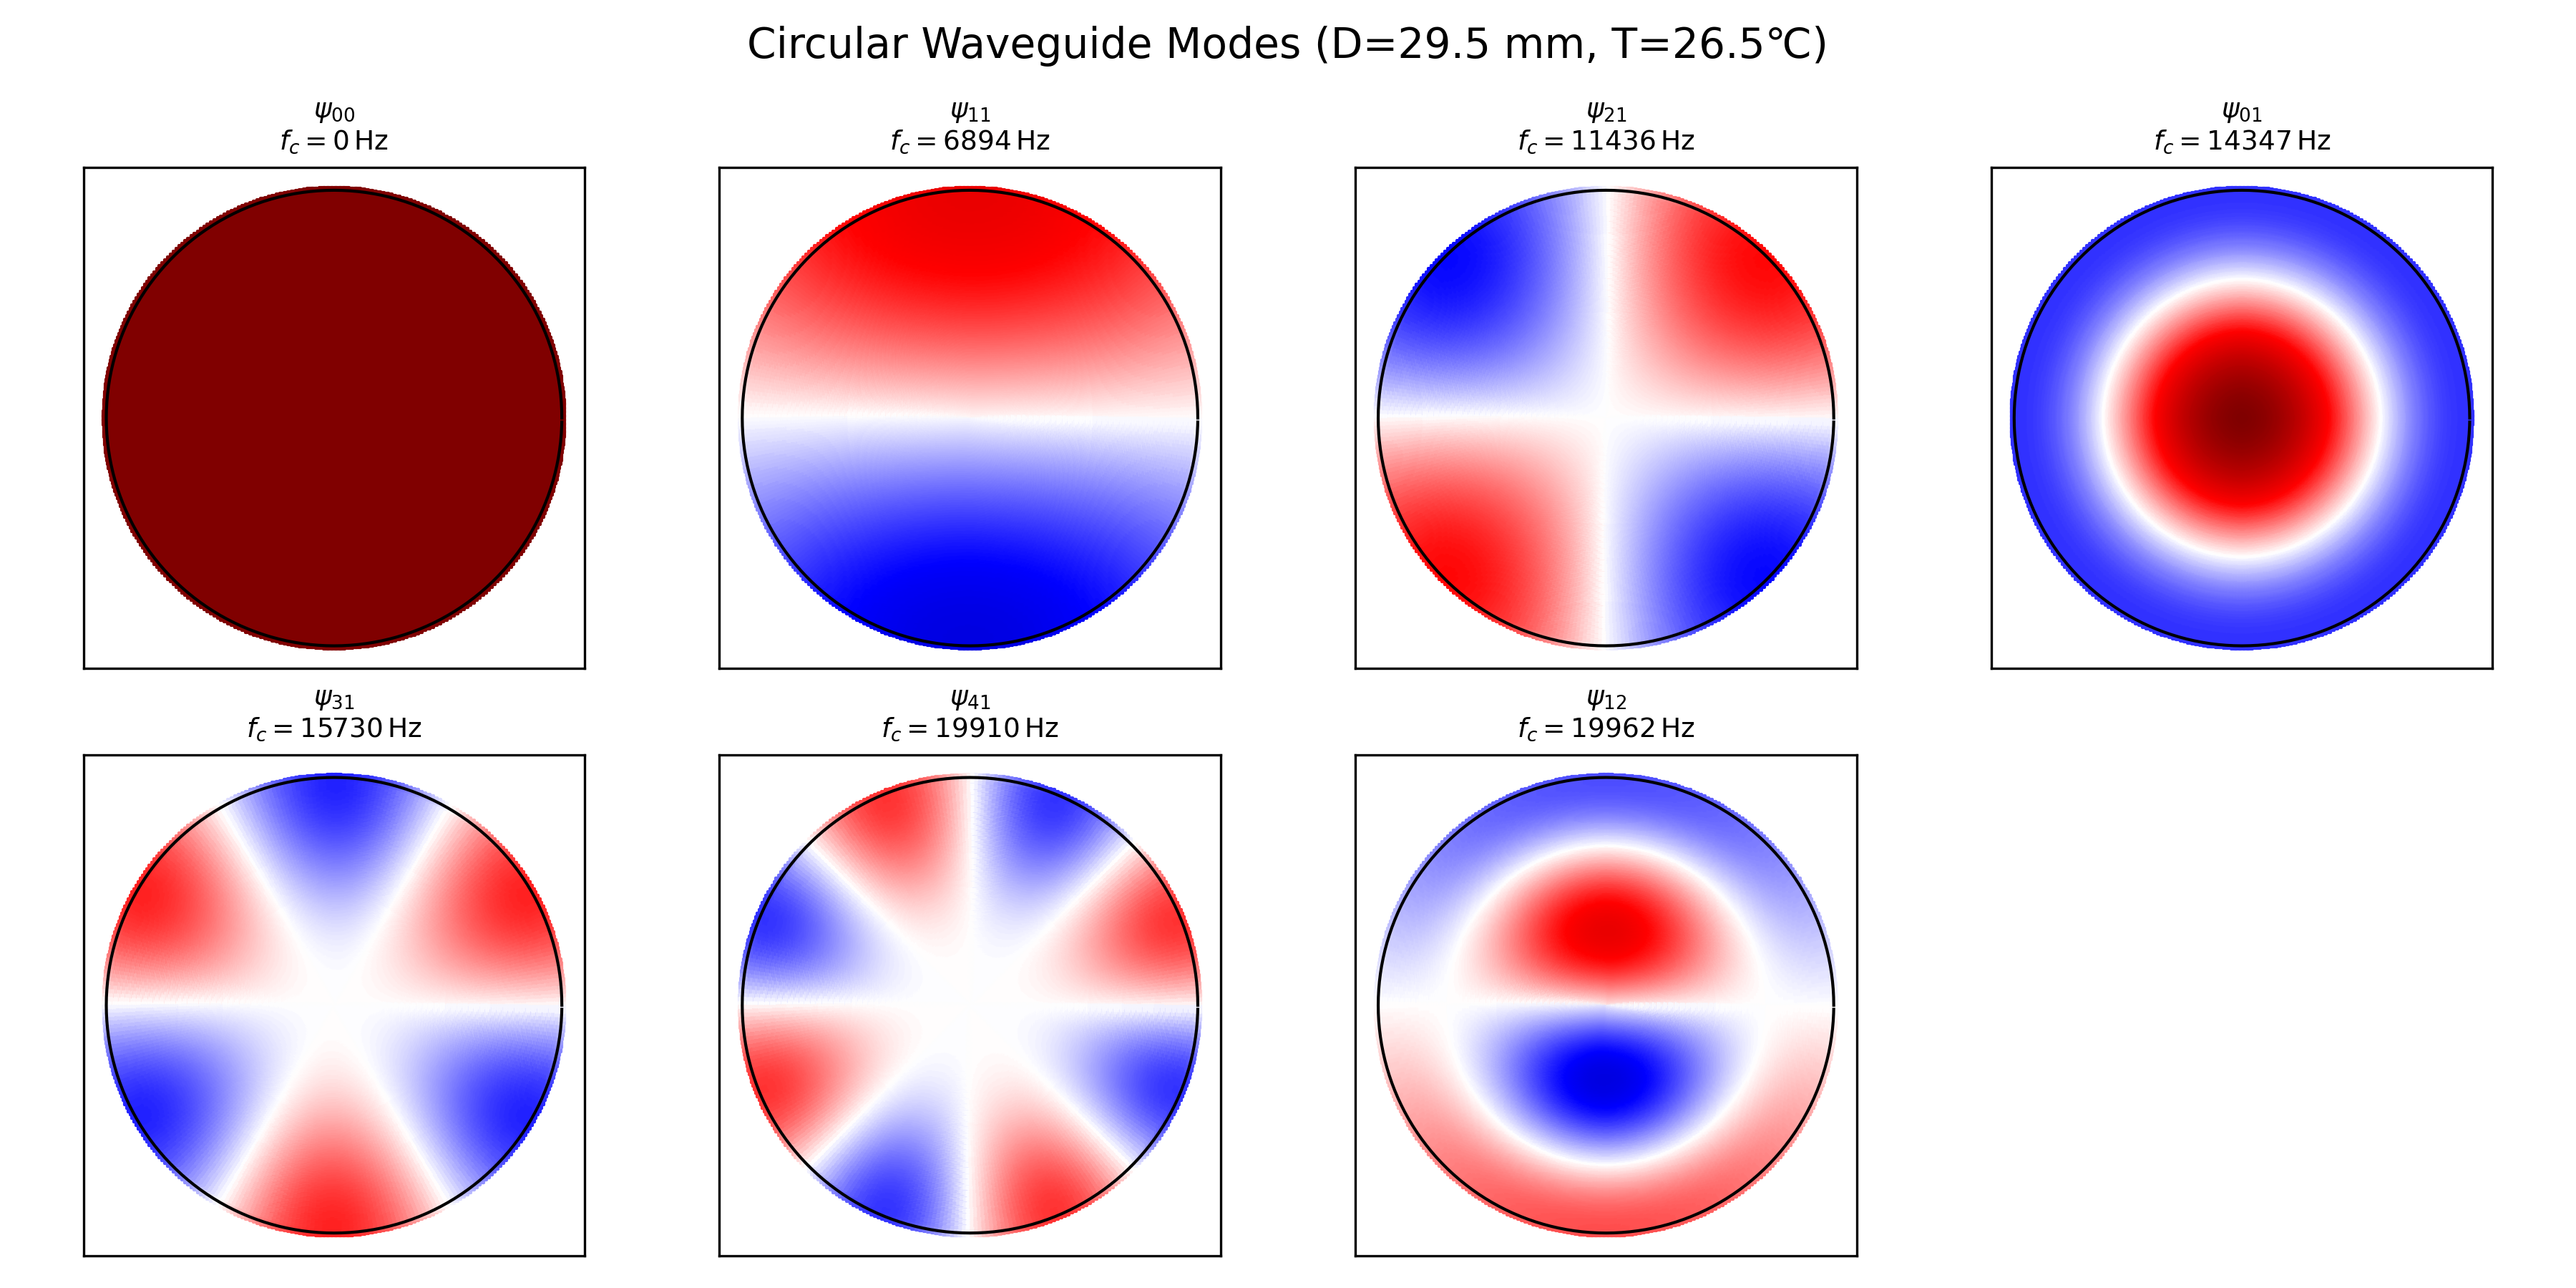
\includegraphics[width=0.8\textwidth]{../02-code/circle_modes.png}
  \caption{圆管部分模态声压分布示例}
  \label{fig:modes}
\end{figure}

%====================================================================
\section{有限长圆管传递函数示例}
脚本 \texttt{tube\_transfer\_compare.py} 计算了两种端面边界(Hard--Hard 与 Hard--Zero)的传递函数,图~\ref{fig:tf} 给出幅度与相位对比。

\begin{figure}[h]
  \centering
  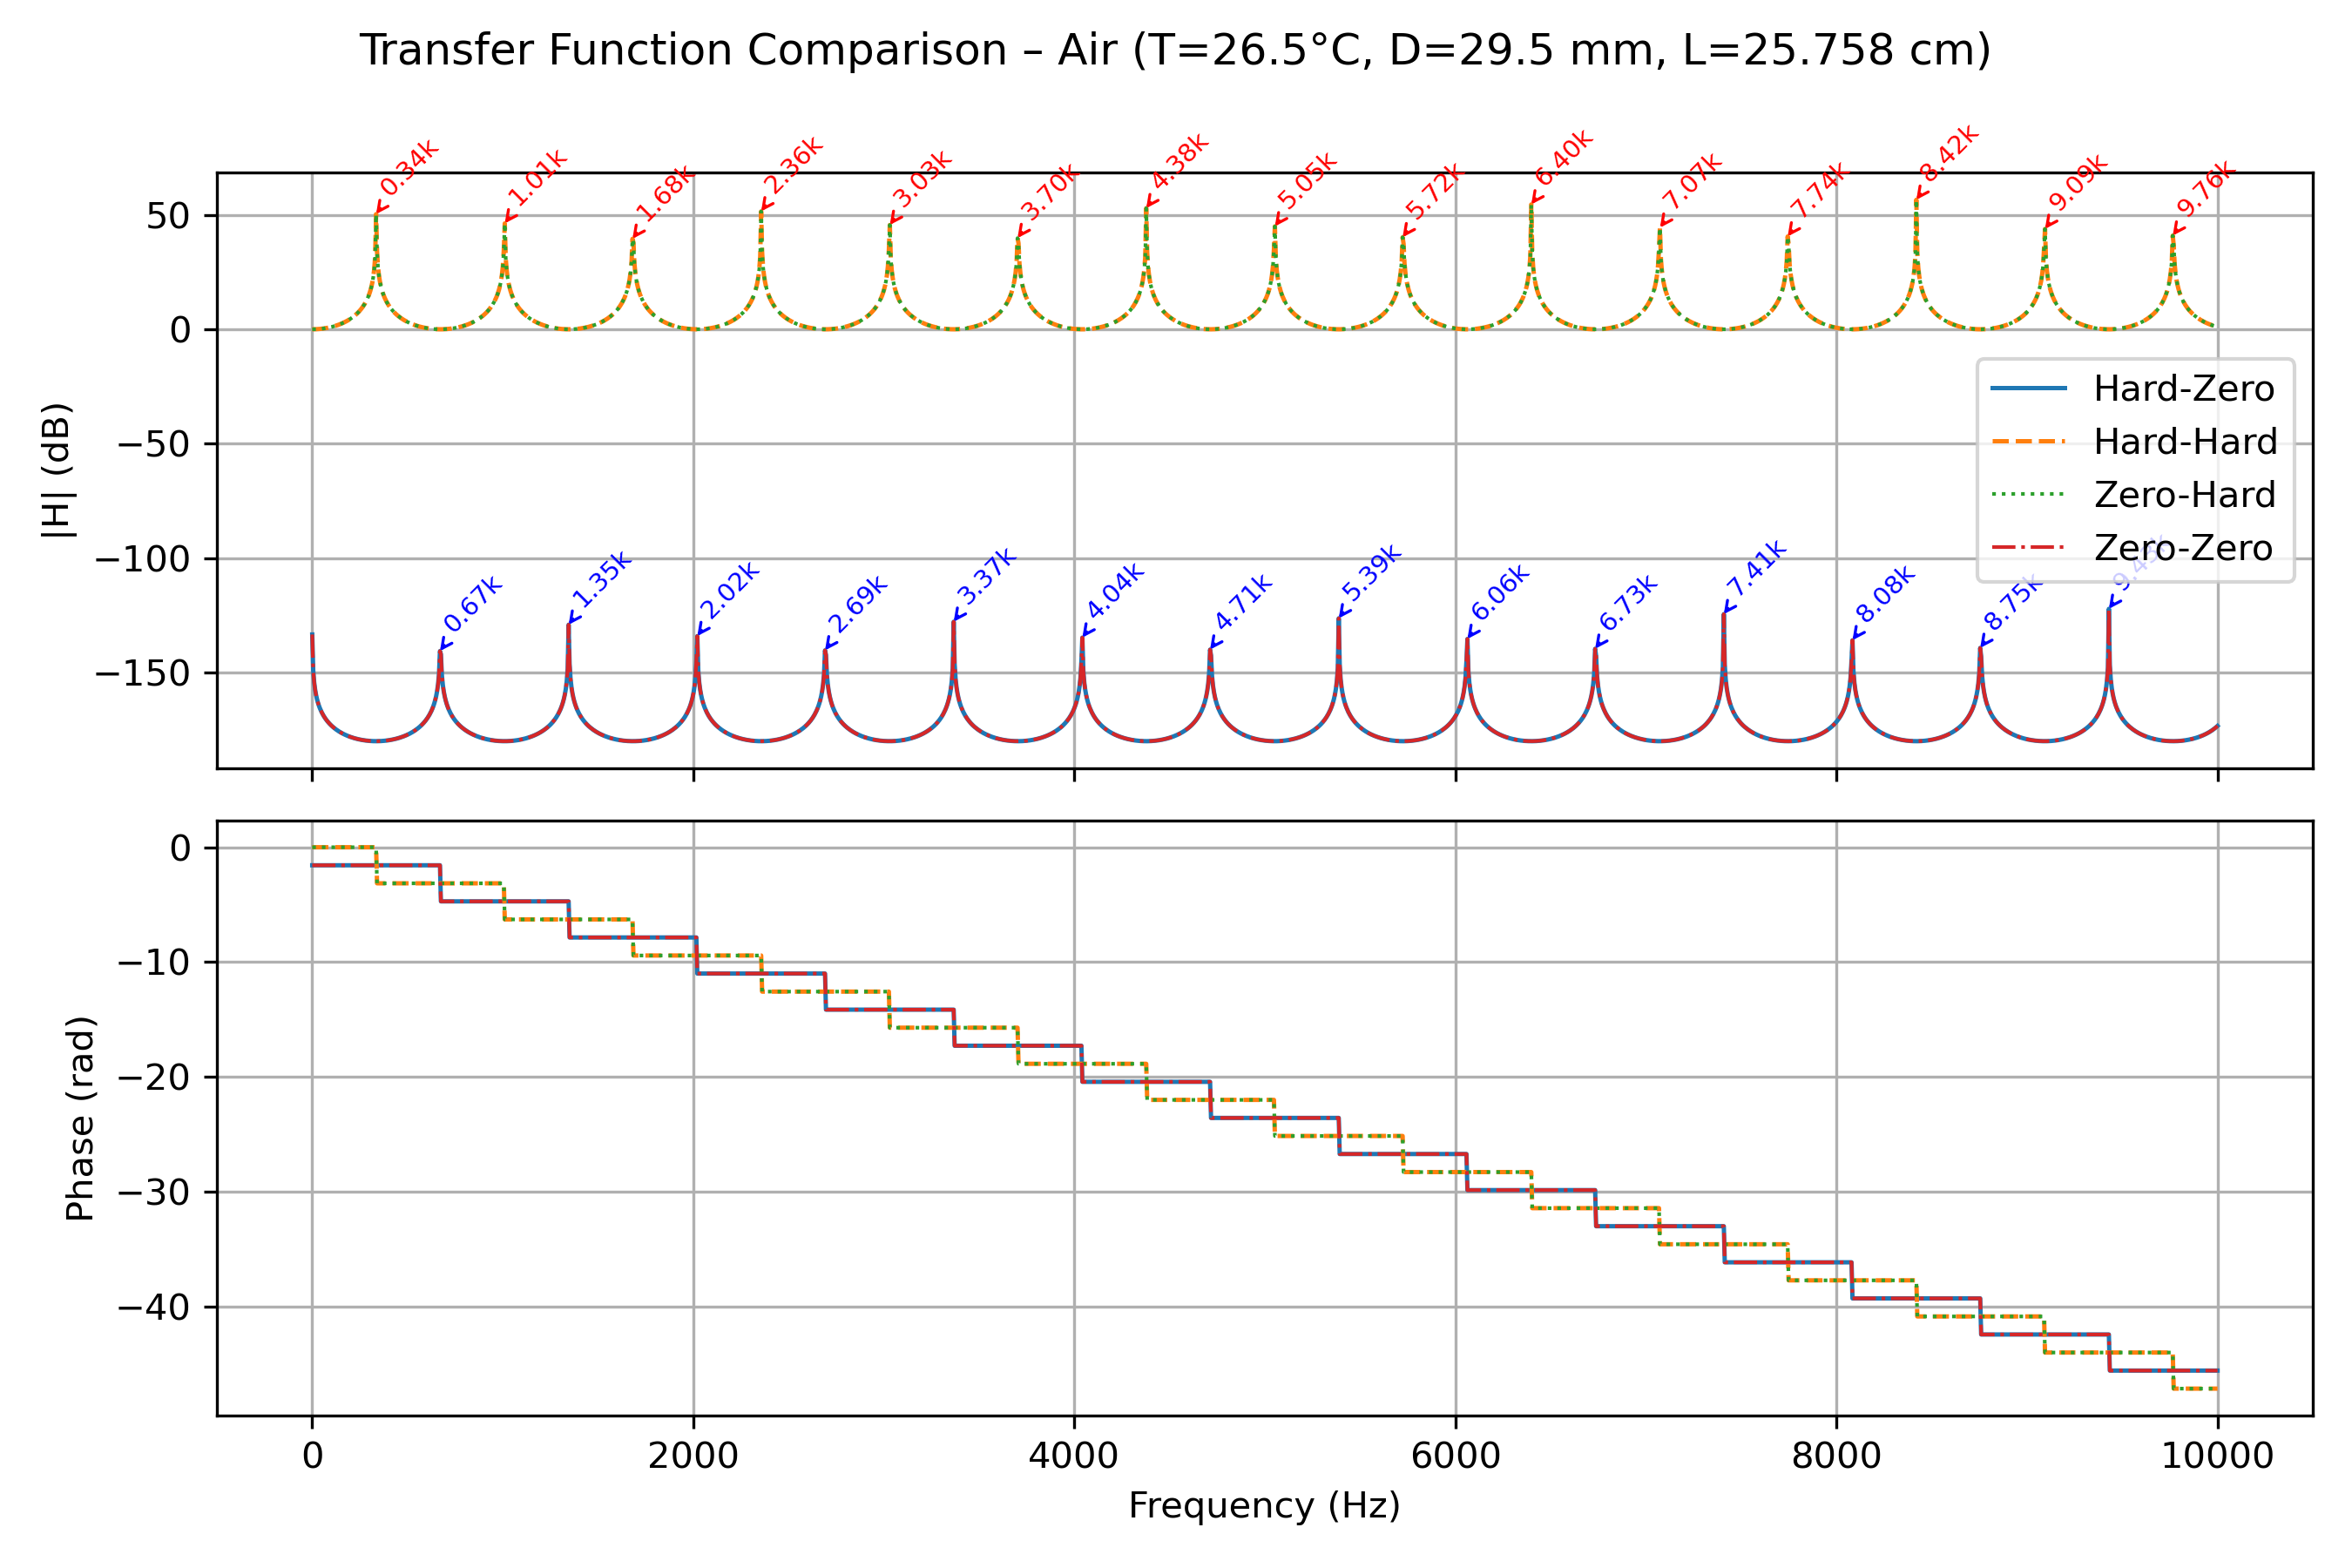
\includegraphics[width=0.9\textwidth]{../02-code/tube_transfer_compare.png}
  \caption{传递函数对比($D=\SI{29.5}{mm}$,$L=\SI{15}{cm}$)}
  \label{fig:tf}
\end{figure}

\paragraph{幅值差异说明} ……(简述原因)。

%====================================================================
\section{结论与展望}
……

%====================================================================
\section*{参考文献}
\begin{enumerate}
  \item P.M. Morse and K.U. Ingard, \emph{Theoretical Acoustics}. Princeton, 1968.
  \item N.H. Fletcher and T.D. Rossing, \emph{The Physics of Musical Instruments}. Springer, 1998.
\end{enumerate}

\end{document} 